
\chapter{Theoretical Introduction}
\label{cha:Theorie}

\section{Characteristics of Muons}

Muons are leptons and belong, together with muon neutrinos, charm and strange quark as well as the corresponding antiparticles, to the second particle generation in the standard model.
They have an energy of $m_{\mu} \approx \qty{105.66}{\mega\electronvolt}/\mathrm{c}^2$\cite{PDG} at rest and therefore a higher mass as electrons with $m_{\mathrm{e}} 
\approx \qty{510.99}{\kilo\electronvolt}/\mathrm{c}^2$\cite{PDG}. The lifetime of the muon has been experimentally established to be $\tau(\mu^{\pm}) = \qty{2.1969e-6}{s} $ \cite{PDG}.\\
Almost all  $(\approx 100 \%)$ muons decay via the following decay channel \cite{PDG}:
\begin{align}
    \mu^{-} &\rightarrow \mathrm{e}^{-} \bar{\nu}_{\mathrm{e}}\nu_{\mu} \\
    \mathrm{resp.} \ \mu^{+} &\rightarrow \mathrm{e}^{+}\nu_{\mathrm{e}} \bar{\nu}_{\mu}.
\end{align}
At earth the biggest source of muons are cosmic high energy hadrons, which react with air particles when reaching the atmosphere and start particle showers.
These particle showers consist of hadronic, electromagnetic and muonic components. The latter ones mostly come from the decay of charged pions, which have a
very short mean lifetime of $\tau_{\pi^{\pm}} \approx \qty{2.6e-8}{\second}$\cite{PDG} and decay via
\begin{align}
    \pi^{-} &\rightarrow \mu^{-} \bar{\nu}_{\mu} (\gamma)\\
    \mathrm{resp.} \ \pi^{+} &\rightarrow \mu^{+} {\nu}_{\mu} (\gamma)
\end{align}
to muons. Usually additional energy is emitted via photons $\gamma$. A schematic view of these particle showers is given in \autoref{fig:Teilchenshower}.\\

\begin{figure}
    \centering
    \includegraphics[width = 0.8\textwidth]{pics/Teilchenkaskade.png}
    \caption{A schematic view of a classical particle shower including hadronic, electromagnetic and muonic components. \cite{WikiKaskade}}
    \label{fig:Teilchenshower}
\end{figure}
Cosmic muons arise at altitudes of approximately $\qty{10}{\kilo\meter}$\cite{MyonenAachen}. Despite energies of a few $\qty{}{\giga\electronvolt}$ and a velocity similiar to the speed of light, cosmic 
muons decay after a few hundred meters. So muons would not be able to reach the earth from a classical point of view. Due to the extremely high velocity, relativistic effects (time delation) have to be taken into account.
From a relativistic point of view, muons travel more than $\qty{10}{\kilo\meter}$ before decaying. This is enough to reach the earth's surface.\\

\section{Mean Lifetime}
In this experiment, the mean lifetime of cosmic muons is to be experimentally established. The mean lifetime is how much time usually passes, before a muon decays. It is the expected value of the 
lifetime distribution, which is derived in the following.\\
In a short time intervall the amount of not decayed particles $N(t)$ falls via the law of radioactive decay:
\begin{equation}
    \mathrm{d}N(t) = - \lambda N(t) \mathrm{d}t,
\end{equation}
with $\lambda$ being the decay constant, which is specific to the decay.\\
After solving the differential equation and integrating, yields an exponential dependency
\begin{equation}
    N(t) = N_0 \exp{(-\lambda t)}.
\end{equation}
The expectation value of this distribution and therefore the mean lifetime is finally given by
\begin{equation}
    \tau = \frac{1}{\lambda}.
\end{equation}

\section{Detection of cosmic Muons}

The muons are detected via a scintillator detector. When a muon enters the scintillator, a light pulse is transmitted to two photomultipliers.
Electrons are then released by means of the photoelectric effect, 
and are accelerated to an electrode via an electric field and release further electrons in the process. This step is repeated a few times until a strong pulse of voltage is created.
The two pulses from the photomultipliers are sent into a coincidence via two discriminators and two variable delays. Since photomultipliers tend to spontaneously fire voltage pulses due to thermal radiation and noise is generated, discriminators
are used to supress this. The coincidence prevents incorrect spontaneous pulses from being registered as signals. Only those pulses are forwarded, which arrive at both inputs at the same time.
This way, only those pulses are accepted which were caused by an event in the scintillator. Since the pulses can have different delays until arriving at the coincidence due to differences in the photomultipliers and cables, variable delays 
can be used to adjust the delays.\\
Finally, three different channels leave from the coincidence. One channel first undergoes a short delay of $\approx \qty{30}{\nano\second}$ and gets transmitted to a monoflip. This converts the pulsed signal into a continuous binary signal.
The monoflop has a normal and an inverted output. A signal would mean TRUE and no signal FALSE. The inverted output of the monoflop is fed into an AND logic together with one of the other two channels of the coincidence to trigger a start of a timer.
The normal output is fed together with the last output of the Coincidence into another AND logic, which is supposed to cause a stop of the stopwatch.
The entry of the muon should start the stopwatch and a second impulse at the decay of the muon should stop it.\\
The delay before the monoflop is necessary so that the signals do not arrive at the AND logics at the same time. This way, a starting and stopping of the timer would not be possible.\\
The monoflop is also used to set a search time after which an event is discarded. This is useful in the case that a muon's energy is too high for it to decay in the scintillator tank. 
The search time is chosen to be about 5 times the expected average lifetime. The amount of start and stop pulses are counted via counters.\\
The time between two pulses is converted into an amplitude via a time-amplitude-converter (TAC). These amplitudes are sorted into different channels by the multi channel analyser and a PC.\\
A schematic view of the detector and the electronics is shown in \autoref{fig:Aufbau}.

\begin{figure}
    \centering
    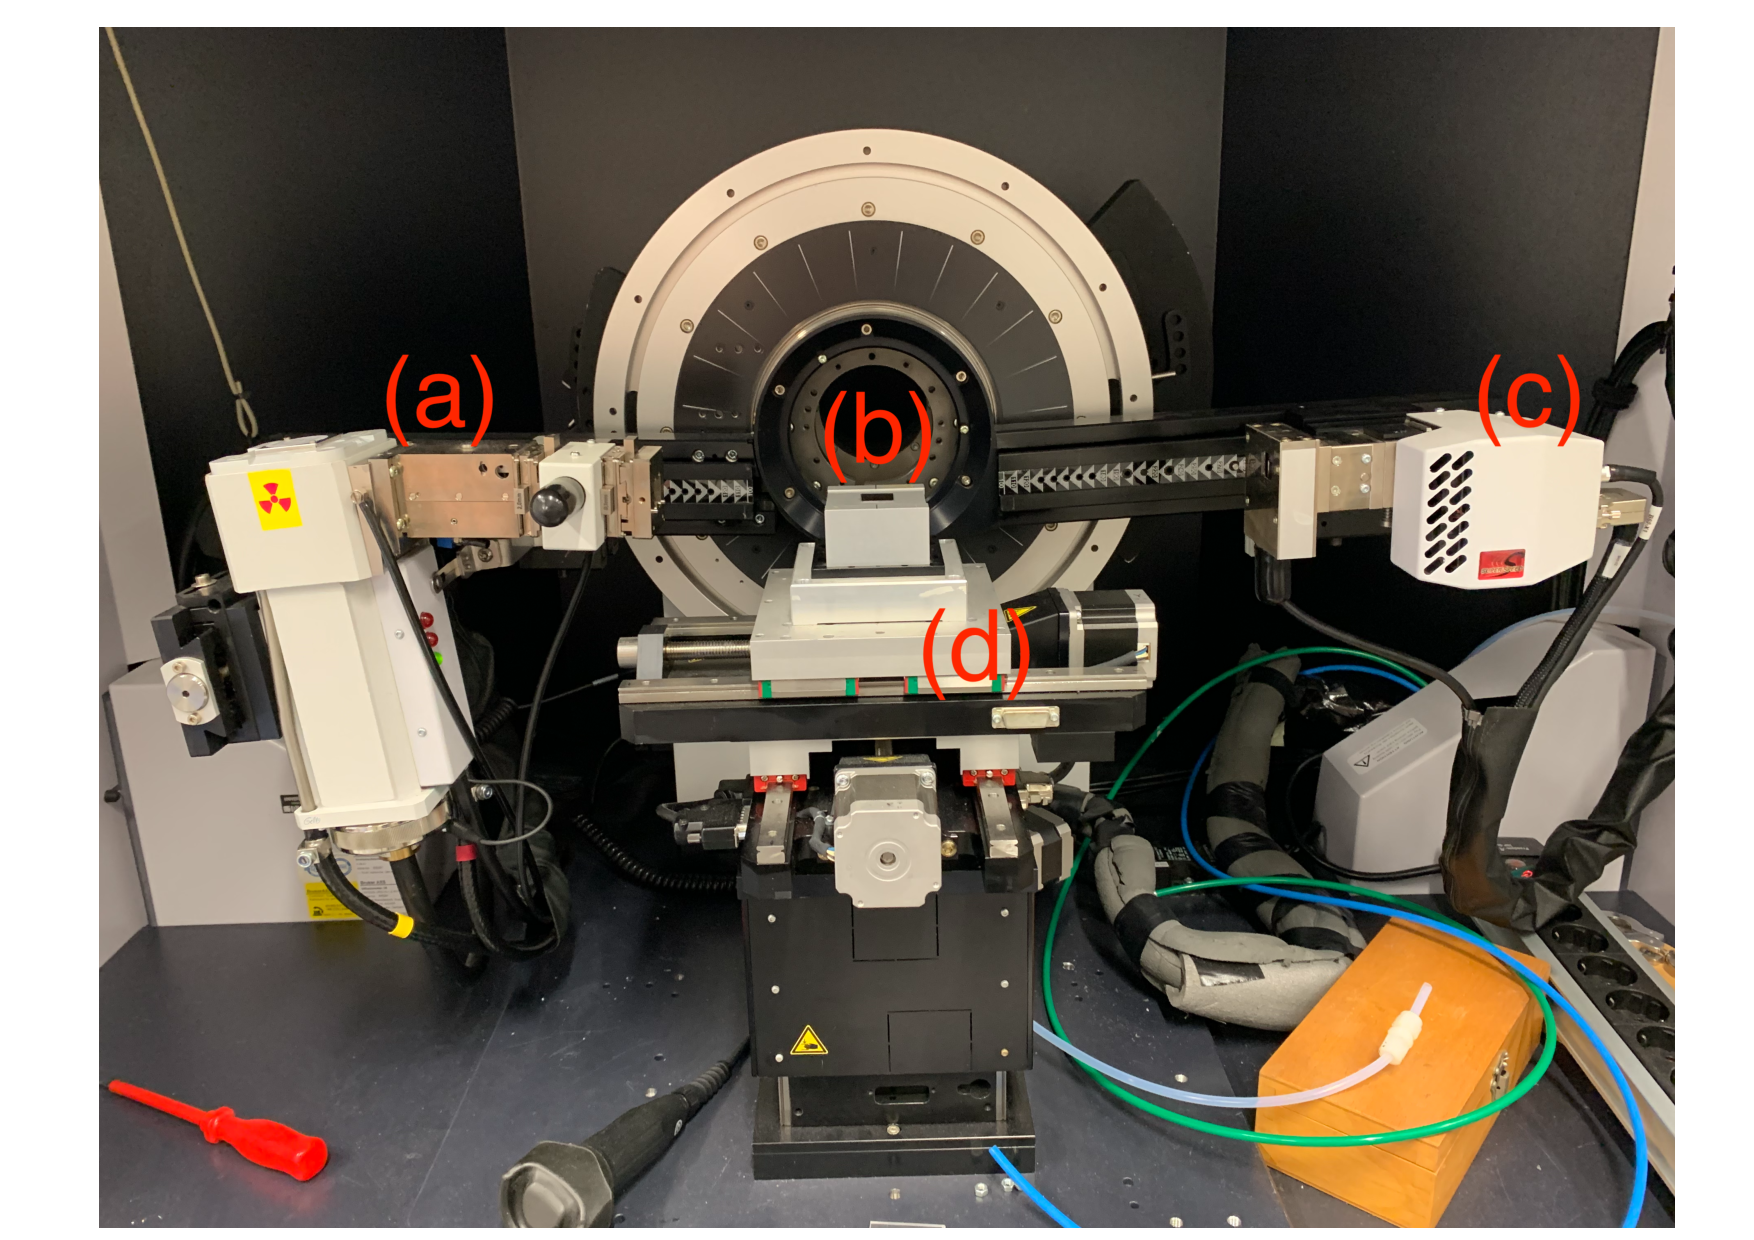
\includegraphics[width = 0.8\textwidth]{pics/Aufbau.png}
    \caption{A schematic view of the experimental aparatus as well as the logic circuit. \cite{v01}}
    \label{fig:Aufbau}
\end{figure}